\documentclass{ximera}

\newcommand{\RR}{\mathbb R}
\renewcommand{\d}{\,d}
\newcommand{\dd}[2][]{\frac{d #1}{d #2}}
\renewcommand{\l}{\ell}
\newcommand{\ddx}{\frac{d}{dx}}
\newcommand{\dfn}{\textbf}
\newcommand{\eval}[1]{\bigg[ #1 \bigg]}


\author{Jason Miller}
\license{Creative Commons 3.0 By-bC}


\outcome{}

\begin{document}
\begin{exercise}


Consider the polar curve $r=\cos(3\theta)$. The graph is show below. 




\begin{image}  
  \begin{tikzpicture}  
    \begin{axis}[  
        xmin=-1.5,  
        xmax=1.5,  
        ymin=-1.5,  
        ymax=1.5,  
        axis lines=center,  
        xlabel=$x$,  
        ylabel=$y$,  
        every axis y label/.style={at=(current axis.above origin),anchor=south},  
        every axis x label/.style={at=(current axis.right of origin),anchor=west},  
      ]  
      \addplot [data cs=polar, very thick, mark=none,fill=fill1,domain=30:90 ,samples=360,smooth] (x, {cos(3*x)}) ;
      \addplot[data cs=polar,blue,domain=0:360,samples=360,smooth, thick] (x,{cos(3*x)});
      
            \end{axis}  
  \end{tikzpicture}  
\end{image} 

We want to set up an integral that expresses the area of the shaded region $S$. 

The area of the region $S$ is 

\[
\int_{\answer{\frac{\pi}{6}}}^{\answer{ \frac{\pi}{3} } } \answer{ \frac{1}{2}(\cos(3\theta))^2   } \d \theta=\answer{ \frac{\pi}{24}}
\]


The entire area enclosed by the curve (all three petals) is $\answer{  \frac{\pi}{8}}$. 


\begin{hint}

Consider a general polar curve $r=f(\theta)$ as below. 


\begin{image}
  \begin{tikzpicture}
\begin{axis}[
axis y line=middle,axis x line=middle,name=myplot,%
			%x=.37\marginparwidth,
			%y=.37\marginparwidth,
			%xtick={-1,1},
			%minor x tick num=1,% 
%			extra x ticks={.33},
%			extra x tick labels={$1/3$},
			%ytick={-1,1},
			%minor y tick num=1,%extra y ticks={-5,-3,...,7},%
			ymin=-.1,ymax=1.1,%
			xmin=-.1,xmax=1.1%
]

\addplot [fill1,fill=fill1,area style, smooth,domain=18:72,samples=30] ({cos(x)*(1+.05*cos(9*x))},{sin(x)*(1+.05*cos(9*x))}) -- (axis cs:0,0) -- cycle;

\addplot [penColor,thick, smooth,domain=0:90,samples=30] ({cos(x)*(1+.05*cos(9*x))},{sin(x)*(1+.05*cos(9*x))});



\draw [thick,penColor,] (axis cs:0,0) -- (axis cs: 0.905831, 0.294322) node [pos=.7,below,rotate=18,black] { $\theta=\alpha$};

\draw [thick,penColor,] (axis cs:0,0) -- (axis cs:0.313792, 0.965751) node [pos=.7,above,rotate=72,black] { $\theta=\beta$};


\draw (axis cs:.8,.85) node { $f(\theta)$};


\end{axis}

\node [right] at (myplot.right of origin) { $0$};
\node [above] at (myplot.above origin) { $\pi/2$};
\end{tikzpicture}
\end{image}


Recall that the area enclosed by a polar curve $r=f(\theta)$ from $\theta=\alpha$ to $\theta=\beta$ is given 

\[
\int_{\alpha}^{\beta} \frac{1}{2} f(\theta)^2 \d \theta
\]


In our case $f(\theta)=\cos(3\theta)$. So we only need to identify the initial angle $\alpha$ and the final angle $\beta$ that bounds our region $S$. 

In order to determine these angles we need to think about how the curve is traced out as $\theta$ varies. 

Let's graph $r=\cos(3\theta)$ on $r$ and $\theta$ axes. 

\begin{image}  
  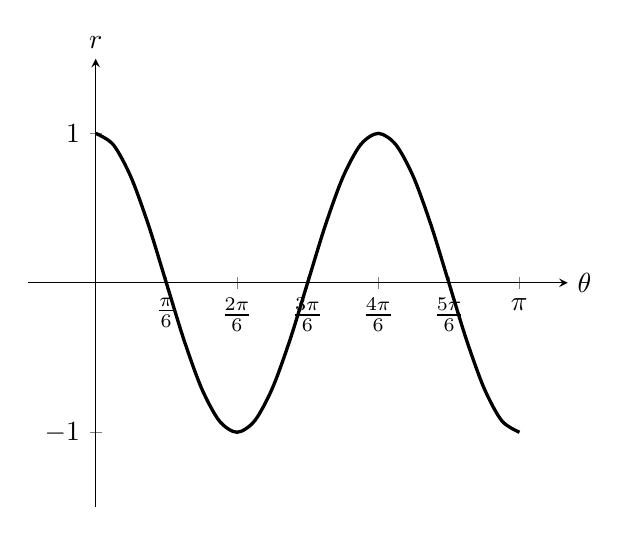
\begin{tikzpicture}  
    \begin{axis}[  
        xmin=-.5,  
        xmax=3.5,  
        ymin=-1.5,  
        ymax=1.5,  
        axis lines=center,  
        xlabel=$\theta$,  
        ylabel=$r$,  
        every axis y label/.style={at=(current axis.above origin),anchor=south},  
        every axis x label/.style={at=(current axis.right of origin),anchor=west},  
       xtick={ .523, 1.047, 1.57, 2.094, 2.62, 3.14  },
       xticklabels={ $\frac{\pi}{6}$, $\frac{2\pi}{6}$, $\frac{3\pi}{6}$, $\frac{4\pi}{6}$, $\frac{5\pi}{6}$, $\pi$ },
            ]  
      \addplot [ very thick, mark=none,domain=0:pi,smooth] {cos(deg(3*x))};
            \end{axis}  
  \end{tikzpicture}  
\end{image} 

This picture shows us clearly how $r$, the distance from the origin varies as $\theta$ varies from $0$ to $\pi$. As $\theta$ goes from $0$ to $\frac{\pi}{6}$ we see that $r$ decreases from $1$ to $0$. This corresponds to the half petal in the 1st quadrant.

 Then as $\theta$ varies from $\frac{\pi}{6}$ to $\frac{\pi}{3}$, we see that $r$ decreases from $0$ to $-1$. Recall that $(r, \theta)$ and $(-r, \theta + \pi)$ refer to the same point so we can always interpret a point with negative radius as one with positive radius where we add $\pi$ to the angle. 

That means as $\theta$ varies from $\frac{\pi}{6}$ to $\frac{\pi}{3}$, we can think of $r$ being positive instead and $\theta$ varying over the interval $\pi + \frac{\pi}{6}$ to $\pi + \frac{\pi}{3}$. 


In order to evaluate the integral, recall the trig identity $sin^2(\theta)=\frac{1-\cos(2\theta)}{2}$. 










\end{hint}

\end{exercise}
\end{document}
